\documentclass[12pt, oneside]{amsart}   	% use "amsart" instead of "article" for AMSLaTeX format
\usepackage[margin=1in]{geometry}                		% See geometry.pdf to learn the layout options. There are lots.
\geometry{letterpaper}                   		% ... or a4paper or a5paper or ... 
%\geometry{landscape}                		% Activate for for rotated page geometry
\usepackage[parfill]{parskip}    		% Activate to begin paragraphs with an empty line rather than an indent
\usepackage{graphicx}				% Use pdf, png, jpg, or eps§ with pdflatex; use eps in DVI mode
								% TeX will automatically convert eps --> pdf in pdflatex		
\usepackage{amssymb,hyperref,float}
% use upquote if available, for straight quotes in verbatim environments
\IfFileExists{upquote.sty}{\usepackage{upquote}}{}

\title{Week 12: R Markdown}
\author{Thomas Elliott}
\date{\today}							% Activate to display a given date or no date

\begin{document}
\maketitle


R Markdown is a type of document that allows you to write papers, memos, articles, etc., using both Markdown and chunks of R code that are run in place. Markdown is a simple formatting syntax for creating HTML, PDF (via \LaTeX), and Word documents. There are a lot of markdown guides online so I won't do a comprehensive overview of markdown. Instead, check out any of the many useful guides for how markdown works. Note that in order to produce PDFs, you'll need to have a TeX engine installed on your computer.

What makes R Markdown a little different is that in addition to formatting, you can also include chunks of R code which get run in place when you ``compile'' the document. The results of these chunks are displayed in place in the final document. RStudio has great support for R Markdown, and writing R Markdown documents in RStudio is incredibly simple.

This is an R Markdown document. Markdown is a simple formatting syntax for authoring HTML, PDF, and MS Word documents. 

When you click the \textbf{Knit} button a document will be generated that includes both content as well as the output of any embedded R code chunks within the document. You can embed an R code chunks be enclosing the lines in 3 or more back tick marks (above the tab key on a US English keyboard). Immediately following the first set of back ticks, you include \texttt{\{r\}} to define the code chunk as an R code chunk (markdown is able to recognize different languages and will apply syntax highlighting appropriately). You can also supply many different options to the code chunk within the braces, including whether to output the lines of code `echo=TRUE`, whether to output the messages generated from commands \texttt{message=TRUE}, or even defining the size of any plots produced by the code \texttt{fig.width=8,fig.height=8}. The R Markdown website (linked below) contains a good primer for the different options available. 

For example, a simple code chunk that prints summary statistics of the \texttt{mtcars} dataset would look like:

\begin{verbatim}
```{r cars}
summary(mtcars)
```
\end{verbatim}

\newpage

And would produce the following in your document:

\begin{verbatim}
##       mpg             cyl             disp             hp       
##  Min.   :10.40   Min.   :4.000   Min.   : 71.1   Min.   : 52.0  
##  1st Qu.:15.43   1st Qu.:4.000   1st Qu.:120.8   1st Qu.: 96.5  
##  Median :19.20   Median :6.000   Median :196.3   Median :123.0  
##  Mean   :20.09   Mean   :6.188   Mean   :230.7   Mean   :146.7  
##  3rd Qu.:22.80   3rd Qu.:8.000   3rd Qu.:326.0   3rd Qu.:180.0  
##  Max.   :33.90   Max.   :8.000   Max.   :472.0   Max.   :335.0  
##       drat             wt             qsec             vs        
##  Min.   :2.760   Min.   :1.513   Min.   :14.50   Min.   :0.0000  
##  1st Qu.:3.080   1st Qu.:2.581   1st Qu.:16.89   1st Qu.:0.0000  
##  Median :3.695   Median :3.325   Median :17.71   Median :0.0000  
##  Mean   :3.597   Mean   :3.217   Mean   :17.85   Mean   :0.4375  
##  3rd Qu.:3.920   3rd Qu.:3.610   3rd Qu.:18.90   3rd Qu.:1.0000  
##  Max.   :4.930   Max.   :5.424   Max.   :22.90   Max.   :1.0000  
##        am              gear            carb      
##  Min.   :0.0000   Min.   :3.000   Min.   :1.000  
##  1st Qu.:0.0000   1st Qu.:3.000   1st Qu.:2.000  
##  Median :0.0000   Median :4.000   Median :2.000  
##  Mean   :0.4062   Mean   :3.688   Mean   :2.812  
##  3rd Qu.:1.0000   3rd Qu.:4.000   3rd Qu.:4.000  
##  Max.   :1.0000   Max.   :5.000   Max.   :8.000
\end{verbatim}

We could also have \texttt{stargazer} output the formatted table directly within our document. To get this to work correctly, you'll have to supply the \texttt{results='asis'} option so that markdown doesn't try to convert the LaTeX code to markdown.

\begin{verbatim}
```{r, results='asis'}
ols<-lm(mpg ~ cyl + hp + wt, data = mtcars)
stargazer(ols,header=FALSE)
```
\end{verbatim}

\newpage

Produces:

\begin{table}[H] \centering 
  \caption{} 
  \label{} 
\begin{tabular}{@{\extracolsep{5pt}}lc} 
\\[-1.8ex]\hline 
\hline \\[-1.8ex] 
 & \multicolumn{1}{c}{\textit{Dependent variable:}} \\ 
\cline{2-2} 
\\[-1.8ex] & mpg \\ 
\hline \\[-1.8ex] 
 cyl & $-$0.942$^{*}$ \\ 
  & (0.551) \\ 
  & \\ 
 hp & $-$0.018 \\ 
  & (0.012) \\ 
  & \\ 
 wt & $-$3.167$^{***}$ \\ 
  & (0.741) \\ 
  & \\ 
 Constant & 38.752$^{***}$ \\ 
  & (1.787) \\ 
  & \\ 
\hline \\[-1.8ex] 
Observations & 32 \\ 
R$^{2}$ & 0.843 \\ 
Adjusted R$^{2}$ & 0.826 \\ 
Residual Std. Error & 2.512 (df = 28) \\ 
F Statistic & 50.171$^{***}$ (df = 3; 28) \\ 
\hline 
\hline \\[-1.8ex] 
\textit{Note:}  & \multicolumn{1}{r}{$^{*}$p$<$0.1; $^{**}$p$<$0.05; $^{***}$p$<$0.01} \\ 
\end{tabular} 
\end{table}

If you are producing a HTML document from R Markdown, you could supply the \texttt{type='html'} argument to \texttt{stargazer}. Unfortunately, there is not a way to get stargazer's pretty tables to work natively in a Word document produced in R Markdown. There are a few packages currently in development to render markdown directly (rather than HTML or \LaTeX code) which should allow Word documents to take advantage of these packages, but I haven't tested them extensively. 

\newpage

\section{Including Plots}

You can also embed plots, for example:

\begin{verbatim}
```{r pressure, echo=FALSE}
plot(mtcars$hp,mtcars$mpg)
```
\end{verbatim}

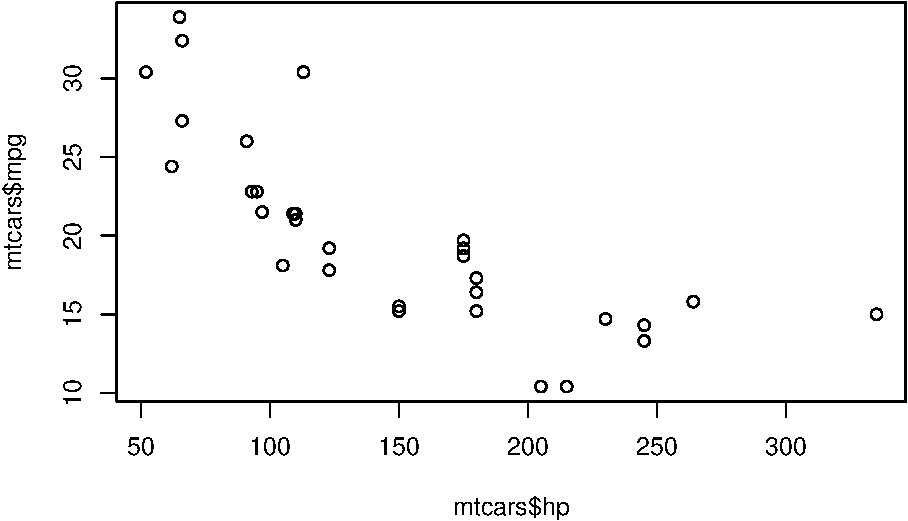
\includegraphics{week11rm_files/figure-latex/pressure-1.pdf}


Here I supplied the argument \texttt{echo = FALSE} which means the code used to generate the figure is not included in the final document. This argument is actually really helpful if you are writing documents for others where the results are important to display, but the code to generate the results are not as important to display for your readers. Theoretically, markdown is powerful enough to allow you to write full academic articles (it can even embed citations and automatically generated a bibliography), in which case you wouldn't want to show any of the actual code, just the generated tables and figures.

For more details on using R Markdown see
\url{http://rmarkdown.rstudio.com}.

\end{document}  